\chapter{Initial Implementation}

For this implementation, we specifically prepared the data for version 15.1.0 of Next.js. In our initial efforts, we concentrated on establishing the foundational components of the system, which included designing the data structure, preparing and preprocessing the data, and configuring both the database and local Large Language Models (LLMs) to develop a functional prototype.

\begin{figure}[H]
\vspace{2pt}
\centering
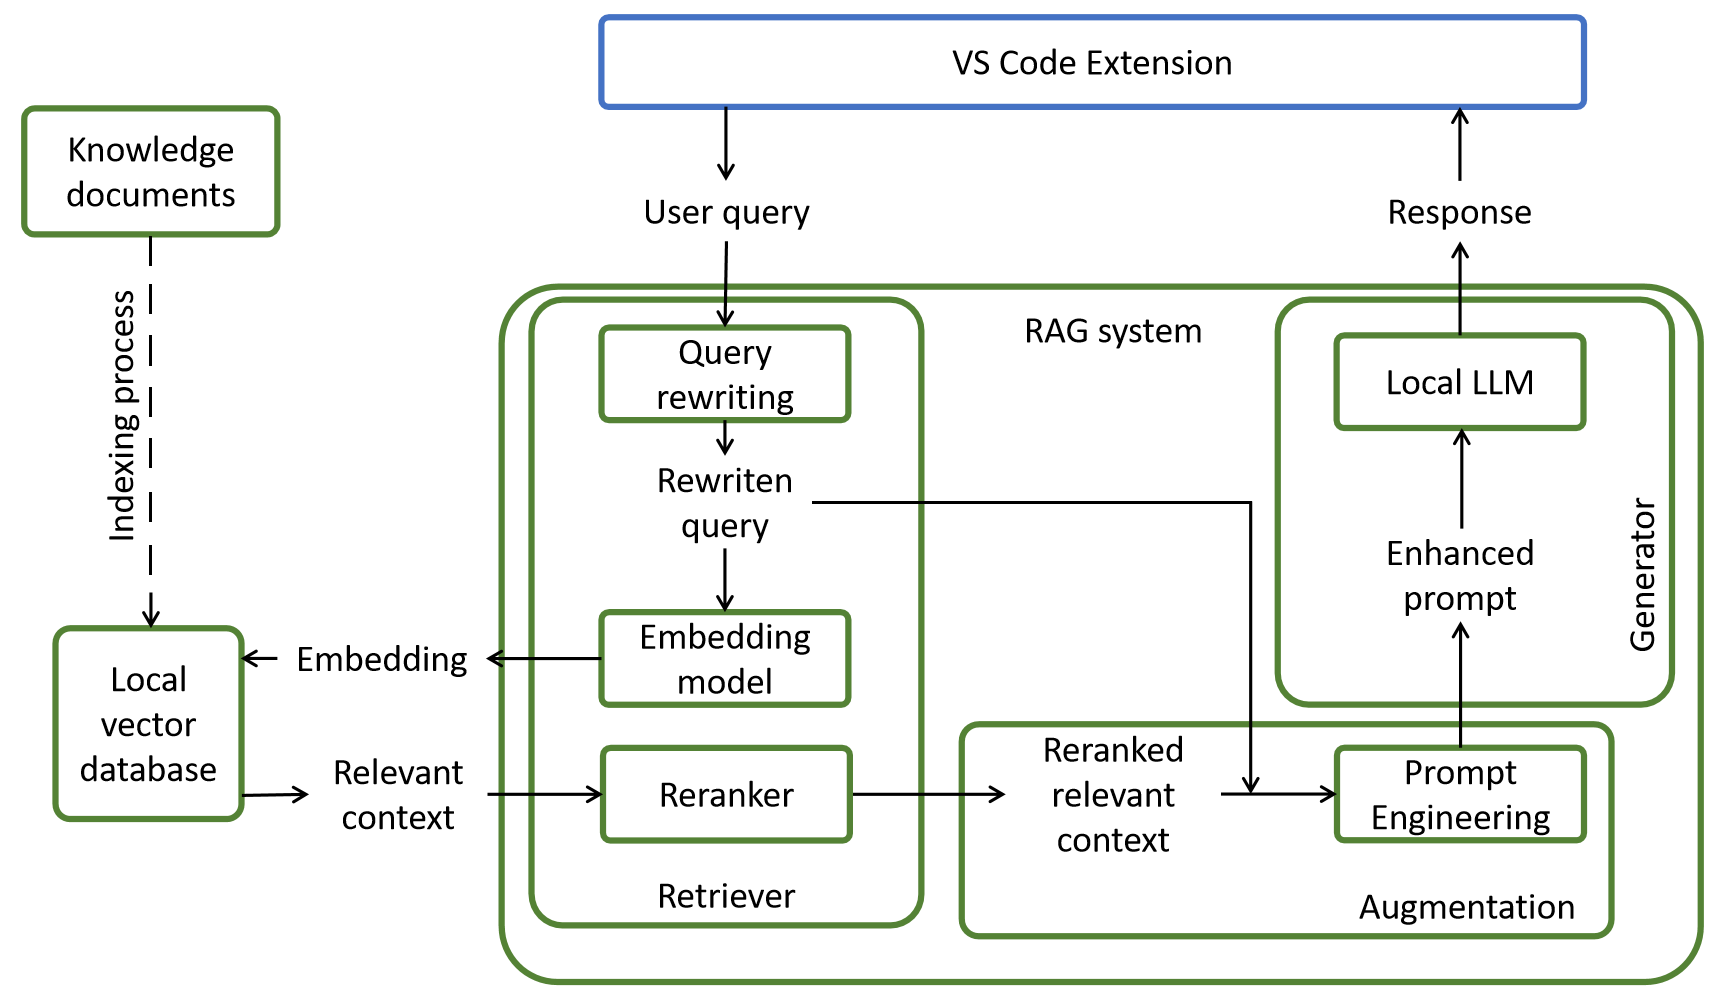
\includegraphics[scale=0.45]{Images/Implement/rag_pipeline.png}
\vspace{5mm}
\caption{Our RAG Pipeline Design}
\end{figure}

\section{Data Structure Design}

Before delving into the structure and preparation of the data, it is important to discuss the data source. Naturally, the official documentation pages of the Next.js framework were our first consideration. Upon examination, the HTML files of the documentation were found to be well-formed and extractable. However, a critical limitation emerged: the official documentation does not maintain a comprehensive version history. The version-selection section often changes its listed versions, making it unreliable for our intended use case.

Our goal is to provide users with the ability to select their current framework version and the version they wish to upgrade or downgrade to. This feature requires reliable and comprehensive documentation for all versions.

Fortunately, we discovered a more reliable data source: the official GitHub repository of the Next.js framework. This repository contains all versions of the framework's documentation in markdown format. These markdown files include useful metadata, explicit sections, and well-organized code snippets, making them ideal for our use case.

\subsection*{Data structure design}

The purpose of our data structure design is to store the Next.js documentation effectively. After analyzing the structure of the markdown files retrieved from the repository, the following key components were identified:

\begin{itemize}
    \item \textbf{Metadata:} Contains information such as:
    \begin{itemize}
        \item \texttt{title}: The title of the documentation page.
        \item \texttt{nav\_title}: The title displayed in the navigation bar.
        \item \texttt{description}: A brief description of the page's content.
        \item \texttt{related}: An optional field containing links to other related documentation pages.
    \end{itemize}
    
    \item \textbf{Text:} The main content of the documentation, divided into sections and subsections using markdown syntax.
    
    \item \textbf{Code Snippets:} Includes:
    \begin{itemize}
        \item \texttt{language}: Programming language used in the snippet (e.g., JavaScript or TypeScript).
        \item \texttt{file}: Indicates the file or component to which the code belongs (Next.js follows a naming convention for files).
        \item \texttt{switcher}: Indicates whether the code snippet has a counterpart in another language (e.g., JavaScript/TypeScript switcher).
        \item \texttt{content}: The actual code content.
    \end{itemize}
    
    \item \textbf{Version History:} A special section explicitly listing major updates to the documentation across versions. However, this section is present in only a small portion of the documentation.
\end{itemize}

\begin{table}[H]
\centering
\label{tab:field_schema_properties}
\begin{tabular}{p{3cm}p{5.5cm}p{5.5cm}l}
\hline
\textbf{Properties}   & \textbf{Description}                                                                 & \textbf{Note}                                                                                                                                         \\ \hline
\texttt{name}         & Name of the field in the collection to create                                        & Data type: String. Mandatory                                                                                                                         \\ \hline
\texttt{dtype}        & Data type of the field                                                              & Mandatory                                                                                                                                             \\ \hline
\texttt{description}  & Description of the field                                                            & Data type: String. Optional                                                                                                                          \\ \hline
\texttt{is\_primary}  & Whether to set the field as the primary key field or not                            & Data type: Boolean (\texttt{true} or \texttt{false}). Mandatory for the primary key field                                                            \\ \hline
\texttt{auto\_id}     & Switch to enable or disable automatic ID (primary key) allocation                   & \texttt{true} or \texttt{false}. Mandatory for primary key field                                                                                     \\ \hline
\texttt{max\_length}  & Maximum byte length for strings allowed to be inserted.                             & {[}1, 65,535{]}. Mandatory for \texttt{VARCHAR} field. Multibyte characters may occupy more than one byte                                            \\ \hline
\texttt{dim}          & Dimension of the vector                                                            & Data type: Integer {[}1, 32,768{]}. Mandatory for dense vector field. Omit for sparse vector field                                                   \\ \hline
\texttt{is\_partition\_key} & Whether this field is a partition-key field                                      & Data type: Boolean (\texttt{true} or \texttt{false})                                                                                                \\ \hline
\end{tabular}
\caption{Field schema properties(Manage Schema\protect\footnotemark).}
\end{table}

\footnotetext{\url{ https://milvus.io/docs/schema.md\#Manage-Schema}}

Based on these components, we designed a schema to organize and store the documentation data efficiently.

\textbf{Collection:} \texttt{nextjs\_docs}

This single collection will store all data, including documents, sections, and code snippets. Each record will represent one of the following:
\begin{itemize}
    \item A \textbf{document}: Represents a top-level page in the documentation.
    \item A \textbf{section}: Represents a subsection within a document.
    \item A \textbf{code snippet}: Represents a code example belonging to a section.
\end{itemize}

\subsection*{Fields in the Schema}

\subsubsection*{Primary Scalar Fields}
\begin{table}[H]
\centering
\label{tab:primary_scalar_fields}
\begin{tabular}{lp{10cm}}
\hline
\textbf{Field Name}          & \textbf{Description}                                                                                      \\ \hline
\texttt{entry\_id} (Primary Key) & Unique identifier for each entry.                                   \\ \hline
\texttt{tag}                  & A tag derived from \texttt{nav\_title} to indicate the subject or topic of the entry. Useful for categorizing and filtering entries by subject. \\ \hline
\texttt{entry\_type}         & Type of entry (\texttt{document}, \texttt{section}, or \texttt{code\_snippet}).                              \\ \hline
\texttt{parent\_id}          & The \texttt{entry\_id} of the parent entry. For:
\begin{itemize}
    \item \textbf{Sections:} Links to the document or other section it belongs to.
    \item \textbf{Code snippets:} Links to the section it belongs to.
\end{itemize} \\ \hline
\texttt{title}               & Title of the document, section, or code snippet.                                           \\ \hline
\texttt{description}         & Description from \texttt{description} metadata.                                          \\ \hline
\texttt{metadata}            & JSON or string field for custom metadata (e.g., programming language, or related links).             \\ \hline
\texttt{version}             & Framework version associated with the entry (e.g., \texttt{"15.1.0"}).                                      \\ \hline
\end{tabular}
\caption{Primary Scalar Fields in the Schema.}
\end{table}

\subsubsection*{Text Fields}
\begin{table}[H]
    \centering
    \begin{tabular}{lp{4cm}p{5cm}}
    \hline
    \textbf{Field Name}                 & \textbf{Index}                  & \textbf{.}          \\ \hline
    \texttt{text\_content}      &  The raw text content (e.g., document or section body). \\ \hline
    \texttt{code\_content}      &  The actual code snippet (only for entries of type \texttt{code\_snippet}). \\ \hline
         & 
    \end{tabular}
    \caption{Caption}
    \label{tab:my_label}
\end{table}

\subsubsection*{Embedding Vectors}
\begin{table}[H]
\centering
\label{tab:embedding_vectors}
\begin{tabular}{lp{4cm}p{5cm}}
\hline
\textbf{Field Name}                 & \textbf{Index}                  & \textbf{Metric}          \\ \hline
\texttt{sparse\_title\_description} & \texttt{SPARSE\_INVERTED\_INDEX} & Inner Product            \\ \hline
\texttt{dense\_text\_content}       & \texttt{HNSW}                   & Cosine Similarity (Dimension: 1024) \\ \hline
\texttt{dense\_code\_snippet}       & \texttt{HNSW}                   & Cosine Similarity (Dimension: 1024) \\ \hline
\end{tabular}
\caption{Embedding Vectors in the Schema.}
\end{table}

\subsubsection*{Partitioning}
\textbf{Field:} \texttt{version}

This field is used to partition entries by \texttt{version}. Partitioning aligns with Milvus's capability for managing partitions, ensuring efficient queries when users specify the framework version.

\section{Data Preparation}

As described in the previous section, our primary data source is the GitHub repository of the Next.js framework. Initially, we developed a crawler that recursively navigated and downloaded resources from the \texttt{docs} and \texttt{errors} folders of the repository. However, this approach faced significant limitations due to GitHub's API rate limits. After careful evaluation, we adopted a more efficient and native method to retrieve data directly from the GitHub repository.

\subsection*{Steps in Data Preparation}

\begin{itemize}
    \item \textbf{Data Acquisition:} 
    To extract the necessary files, we implemented a Python script that utilizes Git's sparse-checkout feature. This approach enabled us to selectively download specific folders, such as \texttt{docs} and \texttt{errors}, corresponding to a particular version tag. The script automates tasks including cloning the repository, configuring sparse-checkout, and checking out the desired version tag.

    \item \textbf{Data Organization:} 
    The retrieved folders and their contents were stored in version-specific directories. For instance, for the version \texttt{v15.1.0}, the directory structure appeared as follows:

% \begin{verbatim}
%     ./v15.1.0/
%         ├── docs/
%         │   ├── 01-app/
%         │   ├── index.mdx
%         │   └── ...
%         ├── errors/
%         │   ├── 404-get-initial-props.mdx
%         │   ├── amp-bind-jsx-alt.mdx
%         │   └── ...
% \end{verbatim}

    This structure provides an organized format, facilitating seamless access and retrieval of documentation resources for different framework versions.

    \item \textbf{Data Integrity Check:} 
    To ensure the integrity and relevance of the dataset, the script included steps to validate and clean the retrieved data. Non-essential files and directories were removed, leaving only the targeted folders and their respective contents. This process ensured that the dataset was well-structured and ready for subsequent preprocessing.
\end{itemize}

\section{Data Preprocessing}

Once the data was acquired and organized, the next critical step was preprocessing it to ensure compatibility with the schema design for effective storage and retrieval. This process involved converting raw markdown files into structured formats through a preprocessing pipeline implemented in Python. The pipeline utilized markdown parsing libraries, embedding models, and structured data processing to extract meaningful information from the documentation.

\subsection*{Key Preprocessing Steps}

\begin{itemize}
    \item \textbf{Metadata Extraction:} 
    The metadata fields, such as \texttt{title}, \texttt{description}, and \texttt{nav\_title}, were extracted from markdown files using the \texttt{frontmatter} library. Additional metadata, such as \texttt{related} links, was included if available. Each document was assigned a unique \texttt{entry\_id} to enable hierarchical referencing within the schema.

    Example code for generating a unique entry ID:
\begin{lstlisting}[language=Python, caption=Generating Unique Entry IDs]
def generate_entry_id(file_path):
    relative_path = os.path.relpath(file_path)
    entry_id = re.sub(r'[^a-zA-Z0-9]', '_', relative_path)
    return entry_id.lower()
\end{lstlisting}

    \item \textbf{Markdown Parsing:} 
    Markdown files were parsed into components such as headings, paragraphs, lists, and code blocks using the \texttt{mistletoe} library. The root token, \texttt{Document}, represented the entire markdown file, while specific tokens such as \texttt{Heading}, \texttt{Paragraph}, and \texttt{List} enabled detailed content extraction while maintaining the document's hierarchy.

    \item \textbf{Content Extraction:} 
    Each token's child elements were recursively processed to capture plain text, inline code, and hyperlinks. For example, \texttt{RawText} tokens represented basic text, \texttt{InlineCode} tokens identified inline code snippets, and \texttt{Link} tokens extracted hyperlink text and URLs.

    \item \textbf{Section Segmentation:} 
    Logical sections were created based on \texttt{Heading} tokens in the markdown. Each section included a title, derived from the heading, and grouped content such as paragraphs, lists, or code blocks. This segmentation maintained the hierarchical structure necessary for efficient data retrieval.

    \item \textbf{Code Snippet Identification:} 
    Code blocks were identified using \texttt{CodeFence} tokens and extracted along with relevant metadata, including the programming language, associated filename, and optional switcher flags. This information linked code snippets to their respective sections and allowed for language-specific queries.

    \item \textbf{Data Structuring:} 
    The extracted sections were structured as dictionaries containing fields such as section title, textual content, and associated code snippets. This data organization was designed to align with the schema in the database for seamless integration.

    \item \textbf{Embedding Preparation:} 
    Text and code content from each section were processed to prepare for embedding generation. Sparse embeddings were used for keyword indexing, while dense embeddings captured semantic meaning, enabling similarity-based queries.

    \item \textbf{Validation and Cleanup:} 
    Parsed sections and their content were validated for completeness and correctness. Empty or incomplete sections were flagged for review, and non-essential formatting artifacts were removed to ensure clean and reliable data.
\end{itemize}

The \texttt{parse\_markdown\_sections} function, implemented using \texttt{mistletoe}, played a central role in these steps by iterating over the document tokens to extract structured information. For instance, a document with headings, paragraphs, and code blocks was transformed into hierarchical sections with associated metadata and content.

Example of parsing and organizing code snippets:
\begin{lstlisting}[language=Python, caption=Code Snippet Parsing]
if isinstance(token, CodeFence):
    code_info = {
        "code": token.children[0].content if token.children else "",
        "language": token.language or "text",
        "filename": filename,
        "switcher": switcher
    }
    current_section["code_snippets"].append(code_info)
\end{lstlisting}

\begin{itemize}
    \item \textbf{Embedding Generation:} 
    Dense and sparse embeddings were generated for both text and code content using a pre-trained embedding model (\texttt{BGEM3EmbeddingFunction}). Dense vectors captured semantic meaning, while sparse vectors indexed key terms for efficient retrieval.

    \item \textbf{Batch Processing and Storage:} 
    Processed entries were saved in batches as CSV files, with fields such as \texttt{entry\_id}, \texttt{entry\_type}, \texttt{text\_content}, and embeddings. This modular strategy supported scalability and efficient handling of large datasets.
\end{itemize}

The preprocessing resulted in 4,714 data entries stored in a CSV file. A total of 481 files were processed, while 97 files were skipped because their content was generated by other files.

\section{Database Setup}

Setting up the database involved configuring Milvus for effective data storage, indexing, and retrieval. This process included deploying Milvus, defining the schema, creating indices, and inserting as well as retrieving data.

\subsection*{Deploying Milvus with Docker Compose}

Milvus was deployed using Docker Compose. After installing Docker, the configuration file was downloaded, and the required containers were initialized. This setup resulted in three key containers:
\begin{itemize}
    \item \textbf{milvus-etcd:} Responsible for managing metadata storage.
    \item \textbf{milvus-minio:} Manages object storage for the system.
    \item \textbf{milvus-standalone:} Handles vector indexing and retrieval services.
\end{itemize}

\subsection*{Installing PyMilvus}

The \texttt{PyMilvus} library was installed to allow programmatic interaction with the Milvus server. To ensure compatibility, the version of \texttt{PyMilvus} matched the Milvus server version (2.4).

\subsection*{Schema Definition and Collection Creation}

As outlined in the data structure design, the database schema was implemented with the collection name \texttt{nextjs\_docs}.

\subsection*{Creating Indices}

To optimize retrieval performance, indices were created for each of the three vector fields:
\begin{itemize}
    \item \textbf{Sparse Index:} Built for the \texttt{sparse\_title\_description} field using an inverted index with inner product (\texttt{IP}) as the metric type.
    \item \textbf{Dense Text Index:} Applied to the \texttt{dense\_text\_content} field using the \texttt{HNSW} algorithm with cosine similarity.
    \item \textbf{Dense Code Index:} Created for the \texttt{dense\_code\_snippet} field, also utilizing the \texttt{HNSW} algorithm with cosine similarity.
\end{itemize}

\subsection*{Inserting Data into the Collection}

The preprocessed data, stored as a CSV file, was read and validated to ensure all data types matched the schema requirements.

\subsection*{Hybrid search implementation}

The hybrid search function was implemented as a prototype to illustrate the retrieval process by integrating sparse and dense embeddings.

\paragraph*{Workflow of Hybrid Search:}

\begin{enumerate}
    \item \textbf{Input and Initialization:}
    Sparse and dense embeddings are provided as inputs, along with weights to balance their influence. Sparse embeddings are processed using the \texttt{sparse\_search} function, while dense embeddings are handled by the \texttt{dense\_text\_search} function.

    \item \textbf{Sparse Search:}
    This step retrieves entries based on keyword relevance. The output includes the entry's metadata and a distance metric.

    \item \textbf{Dense Search:}
    This step retrieves entries based on semantic similarity, outputting the entry's metadata and a distance metric.

    \item \textbf{Combining Results:}
    The results from sparse and dense searches are merged using \texttt{entry\_id} as the common key. A combined score is calculated for each entry:
    \[
    \text{Combined Score} = (\text{Sparse Distance} \times \text{Sparse Weight}) + (\text{Dense Distance} \times \text{Dense Weight})
    \]
    If an entry is missing in either result, its corresponding distance is set to zero.

    \item \textbf{Sorting and Limiting Results:}
    The entries are ranked by their combined scores in descending order. The top \texttt{limit} results are returned, demonstrating the hybrid retrieval process.
\end{enumerate}

\section{Local LLMs setup}

In the development of RAG systems, the choice of a robust and secure LLM is critical for achieving high-quality responses and ensuring data privacy. To support our RAG pipeline, we installed and configured Ollama\footnote{Ollama - \url{https://ollama.com/}}, a platform specifically designed to facilitate the deployment of pre-trained language models on local infrastructure. This section describes the setup and integration of Ollama into our system.

\textbf{Setup Ollama}

The setup process begins by installing the Ollama application, which is compatible with various operating systems including Windows, macOS, and Linux. Once installed, Ollama provides a straightforward interface to download and configure pre-trained models without requiring fine-tuning.

The installation of specific models is conducted via the command prompt or terminal, with available models conveniently listed on \url{https://ollama.com/search}.
The command to install a model is \verb|ollama pull <model_name>|.

Once a model is installed, it is stored locally, ensuring a high level of data privacy and security — an essential feature for applications dealing with sensitive or proprietary information. To test the model, we can use the command \verb|ollama run <model_name>| .

Furthermore, the platform’s lightweight design enhances compatibility across a variety of hardware configurations, making it particularly suitable for environments with limited computational resources. This flexibility makes Ollama an optimal choice for deploying local LLMs in diverse use cases.

% For instance, installing a model such as Meta's llama3.2  can be accomplished with the following command:

% \begin{verbatim}
% ollama pull llama3.2
% \end{verbatim}



% This command downloads the desired model and sets up the necessary configurations, enabling immediate usage. Ollama’s design ensures that users do not need to worry about manual configurations, as the system handles all dependencies and environment settings.




\textbf{Integration with the RAG System}

To integrate Ollama into the RAG workflow, we use the Ollama API for direct interaction with the locally installed models. The endpoint for the API is:

POST \url{http://localhost:11434/api/generate}

The POST request body should be in JSON format, specifying the desired model and the prompt to be processed. An example request body is shown below:

\begin{verbatim}
        {
          "model": "qwen",
          "prompt": "What is RAG?"
        }
\end{verbatim}

The API provides a straightforward and efficient method for passing queries and receiving responses from the model. 

Alternatively, Ollama models can also be integrated using the Python library LangChain\footnote{LangChain - \url{https://python.langchain.com/docs/introduction/}}. With LangChain, the locally installed Ollama models can be accessed and utilized as part of a more comprehensive pipeline, allowing for advanced customization and ease of interaction. This flexibility enables developers to build robust RAG systems that leverage the full potential of Ollama's capabilities while adapting to diverse use cases.







